\tikzstyle{busmaster} = [draw=red, fill=blue!20, thick, rectangle,
  rounded corners, inner sep=0.2cm]

\tikzstyle{busunit} = [draw=red, fill=blue!20, thick,
  rectangle, rounded corners, inner sep=0.2cm]

\tikzstyle{bus} = [draw=black, fill=white, thick, rectangle, minimum
  width=5cm, minimum height=1pt]

\begin{figure}[hbt!]
  \begin{center}
    \subfigure[Prije početka komunikacije]{
      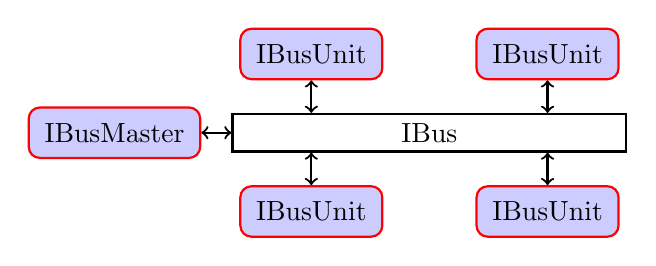
\begin{tikzpicture}
        \node [bus]       (bus)                    {IBus};
        \node [busmaster] (busmaster) at (-4.0, 0) {IBusMaster};
        \node [busunit]   (busunit1)  at (-1.5, 1) {IBusUnit};
        \node [busunit]   (busunit2)  at ( 1.5, 1) {IBusUnit};
        \node [busunit]   (busunit3)  at (-1.5,-1) {IBusUnit};
        \node [busunit]   (busunit4)  at ( 1.5,-1) {IBusUnit};

        \draw[<->,thick] (busmaster.east) -- (bus.west);
        \draw[<->,thick] (busunit1.south) -- (busunit1.south |- bus.north);
        \draw[<->,thick] (busunit2.south) -- (busunit2.south |- bus.north);
        \draw[<->,thick] (busunit3.north) -- (busunit3.north |- bus.south);
        \draw[<->,thick] (busunit4.north) -- (busunit4.north |- bus.south);
      \end{tikzpicture}
    }
    \subfigure[IBus.requestBusWrite(IBusMaster,Address,Data)]{
      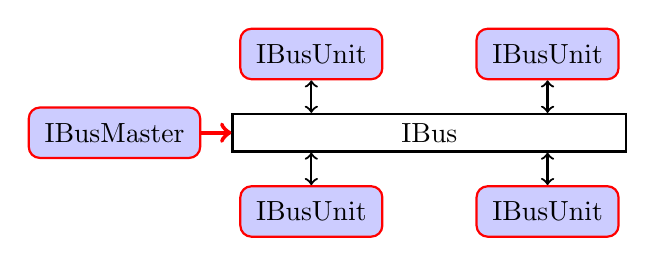
\begin{tikzpicture}
        \node [bus]       (bus)                    {IBus};
        \node [busmaster] (busmaster) at (-4.0, 0) {IBusMaster};
        \node [busunit]   (busunit1)  at (-1.5, 1) {IBusUnit};
        \node [busunit]   (busunit2)  at ( 1.5, 1) {IBusUnit};
        \node [busunit]   (busunit3)  at (-1.5,-1) {IBusUnit};
        \node [busunit]   (busunit4)  at ( 1.5,-1) {IBusUnit};

        \draw[->,ultra thick,color=red] (busmaster.east) -- (bus.west);
        \draw[<->,thick] (busunit1.south) -- (busunit1.south |- bus.north);
        \draw[<->,thick] (busunit2.south) -- (busunit2.south |- bus.north);
        \draw[<->,thick] (busunit3.north) -- (busunit3.north |- bus.south);
        \draw[<->,thick] (busunit4.north) -- (busunit4.north |- bus.south);
      \end{tikzpicture}
    }
    \subfigure[IBusUnit.requestBusUnitWrite(IBus,TranslatedAddress,Data)]{
      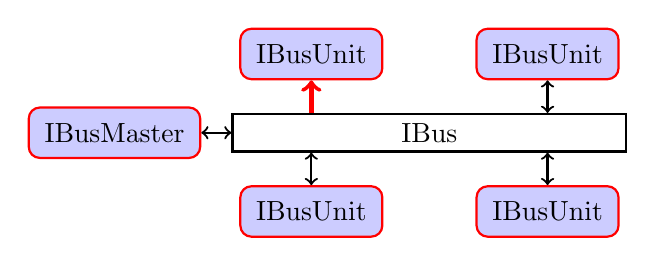
\begin{tikzpicture}
        \node [bus]       (bus)                    {IBus};
        \node [busmaster] (busmaster) at (-4.0, 0) {IBusMaster};
        \node [busunit]   (busunit1)  at (-1.5, 1) {IBusUnit};
        \node [busunit]   (busunit2)  at ( 1.5, 1) {IBusUnit};
        \node [busunit]   (busunit3)  at (-1.5,-1) {IBusUnit};
        \node [busunit]   (busunit4)  at ( 1.5,-1) {IBusUnit};

        \draw[<->,thick] (busmaster.east) -- (bus.west);
        \draw[<-,ultra thick, color=red] (busunit1.south) --
        (busunit1.south |- bus.north);
        \draw[<->,thick] (busunit2.south) -- (busunit2.south |- bus.north);
        \draw[<->,thick] (busunit3.north) -- (busunit3.north |- bus.south);
        \draw[<->,thick] (busunit4.north) -- (busunit4.north |- bus.south);
      \end{tikzpicture}
    }
    \subfigure[IBus.busUnitWriteCallback(IBusUnit,TranslatedAddress)]{
      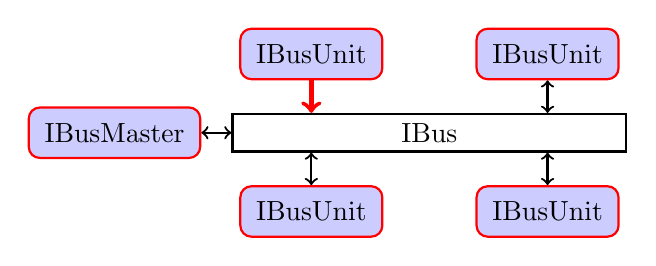
\begin{tikzpicture}
        \node [bus]       (bus)                    {IBus};
        \node [busmaster] (busmaster) at (-4.0, 0) {IBusMaster};
        \node [busunit]   (busunit1)  at (-1.5, 1) {IBusUnit};
        \node [busunit]   (busunit2)  at ( 1.5, 1) {IBusUnit};
        \node [busunit]   (busunit3)  at (-1.5,-1) {IBusUnit};
        \node [busunit]   (busunit4)  at ( 1.5,-1) {IBusUnit};

        \draw[<->,thick] (busmaster.east) -- (bus.west);
        \draw[->,ultra thick, color=red] (busunit1.south) --
        (busunit1.south |- bus.north);
        \draw[<->,thick] (busunit2.south) -- (busunit2.south |- bus.north);
        \draw[<->,thick] (busunit3.north) -- (busunit3.north |- bus.south);
        \draw[<->,thick] (busunit4.north) -- (busunit4.north |- bus.south);
      \end{tikzpicture}
    }
    \subfigure[IBusMaster.busWriteCallback(IBus,Address)]{
      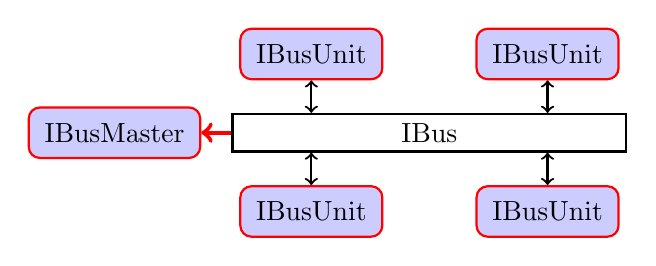
\begin{tikzpicture}
        \node [bus]       (bus)                    {IBus};
        \node [busmaster] (busmaster) at (-4.0, 0) {IBusMaster};
        \node [busunit]   (busunit1)  at (-1.5, 1) {IBusUnit};
        \node [busunit]   (busunit2)  at ( 1.5, 1) {IBusUnit};
        \node [busunit]   (busunit3)  at (-1.5,-1) {IBusUnit};
        \node [busunit]   (busunit4)  at ( 1.5,-1) {IBusUnit};

        \draw[<-,ultra thick,color=red] (busmaster.east) -- (bus.west);
        \draw[<->,thick] (busunit1.south) -- (busunit1.south |- bus.north);
        \draw[<->,thick] (busunit2.south) -- (busunit2.south |- bus.north);
        \draw[<->,thick] (busunit3.north) -- (busunit3.north |- bus.south);
        \draw[<->,thick] (busunit4.north) -- (busunit4.north |- bus.south);
      \end{tikzpicture}
    }
  \end{center}

  \caption{Protokol za sabirnicu (pisanje); slično vrijedi i za
    čitanje samo što se onda podaci prenose preko callback metoda}
  \label{bus_protocol}
\end{figure}
